\documentclass[11pt,a4paper]{article}
\usepackage[margin=18mm]{geometry}
\usepackage{amsmath,amssymb,mathtools}
\usepackage{booktabs,array,enumitem}
\usepackage[dvipsnames]{xcolor}
\usepackage{graphicx,listings,tikz}
\usetikzlibrary{arrows.meta,positioning}
\usepackage[most]{tcolorbox}
\usepackage{hyperref}
\hypersetup{colorlinks=true,urlcolor=MidnightBlue,linkcolor=MidnightBlue}
\setlength{\parindent}{0pt}\setlength{\parskip}{4pt}
\newcommand{\course}{PHY4605 Computational Methods in Physics}
\newcommand{\units}[1]{\,\mathrm{#1}}
\newtcolorbox{keybox}{colback=RoyalBlue!5,colframe=RoyalBlue!65!black,boxrule=.7pt,arc=2mm}
\newtcolorbox{checkbox}{colback=ForestGreen!5,colframe=ForestGreen!55!black,boxrule=.7pt,arc=2mm}
\newtcolorbox{aibox}{colback=BurntOrange!7,colframe=BurntOrange!80!black,boxrule=.7pt,arc=2mm}
\lstdefinestyle{matlabstyle}{language=Matlab,basicstyle=\ttfamily\footnotesize,keywordstyle=\color{RoyalBlue!75!black},commentstyle=\color{ForestGreen!55!black},stringstyle=\color{BurntOrange!80!black},numbers=left,numberstyle=\scriptsize\color{black!50},numbersep=5pt,frame=single,rulecolor=\color{RoyalBlue!25},backgroundcolor=\color{RoyalBlue!3},showstringspaces=false,columns=fullflexible,keepspaces=true,breaklines=true}
\begin{document}
{\large\textsc{\course}}\\[-2pt]
{\small Learning Note \textbar\ Week 1}\par\vspace{4pt}
{\LARGE\bfseries Physics to Arrays and Plots}\par\vspace{3pt}
\textit{Use one familiar vertical-motion model to turn physical quantities into a reproducible MATLAB graph.}
\begin{keybox}\textbf{Physical question.} A ball is launched straight upward. How does its vertical position change during the first four seconds after launch, and how can a MATLAB array show that motion?\end{keybox}
\section*{Core learning outcomes}
\begin{enumerate}[nosep,leftmargin=5mm]
\item identify the physical question, model variables, parameters, and units;
\item make and inspect a time array, then evaluate a familiar equation at every stored time; and
\item predict, plot, validate, and interpret the position--time graph.
\end{enumerate}
\section*{How to use this note}
Read each physical claim before the MATLAB fragment below it. Pause at prediction and trace prompts before running the lecture demonstration. The goal is not to memorise punctuation: it is to keep the model, units, calculation, graph, and check connected.
\begin{keybox}\textbf{Week 1 bridge.} One analytical equation is already familiar. The new computational idea is that an array gives the equation many input times, so MATLAB can return many positions and make the motion visible.\end{keybox}
\section*{1. The computational-physics cycle}
Computation is a controlled experiment on a physical model. A reliable graph follows the same chain every time.
\begin{center}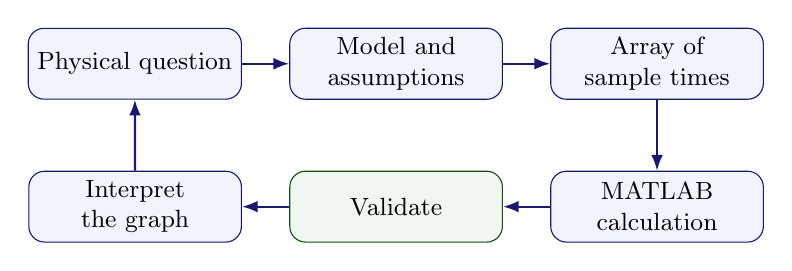
\begin{tikzpicture}[node distance=9mm and 6mm,every node/.style={font=\small,align=center},box/.style={draw=MidnightBlue,rounded corners=2mm,fill=RoyalBlue!7,minimum width=27mm,minimum height=9mm},check/.style={draw=ForestGreen!55!black,rounded corners=2mm,fill=ForestGreen!7,minimum width=27mm,minimum height=9mm},arrow/.style={-{Latex[length=2mm]},thick,MidnightBlue}]
\node[box] (q) {Physical question}; \node[box,right=of q] (m) {Model and\\assumptions}; \node[box,right=of m] (a) {Array of\\sample times};
\node[box,below=of a] (c) {MATLAB\\calculation}; \node[check,left=of c] (v) {Validate}; \node[box,left=of v] (i) {Interpret\\the graph};
\draw[arrow] (q)--(m); \draw[arrow] (m)--(a); \draw[arrow] (a)--(c); \draw[arrow] (c)--(v); \draw[arrow] (v)--(i); \draw[arrow] (i)--(q);\end{tikzpicture}\end{center}
For this week, the physical model is analytical. We are sampling a known expression at many times so that its physical trend can be inspected.
\section*{2. Physical picture, model, and units}
Choose upward as positive. Neglect air resistance and take gravitational acceleration to be constant. The vertical position is
\[y(t)=y_0+v_0t-\frac{1}{2}gt^2.\]
In words: \emph{position equals the starting position plus the upward launch contribution minus the downward gravity contribution}. The last term has a minus sign because gravity points downward in our coordinate direction.
\begin{center}\small\begin{tabular}{>{\raggedright\arraybackslash}p{.20\linewidth}>{\raggedright\arraybackslash}p{.24\linewidth}>{\raggedright\arraybackslash}p{.42\linewidth}}\toprule
\textbf{Physics symbol} & \textbf{MATLAB name} & \textbf{Meaning and unit}\\ \midrule
$y(t)$ & \texttt{y\_m} & vertical position, m\\ $t$ & \texttt{t\_s} & time or time array, s\\ $y_0$ & \texttt{y0\_m} & starting position, m\\ $v_0$ & \texttt{v0\_mps} & upward launch velocity, m s$^{-1}$\\ $g$ & \texttt{g\_mps2} & gravity magnitude, m s$^{-2}$\\ \bottomrule\end{tabular}\end{center}
The locked values are $y_0=0\units{m}$, $v_0=20\units{m\,s^{-1}}$, and $g=9.81\units{m\,s^{-2}}$. Time will run from $0$ to $4\units{s}$.
\begin{checkbox}\textbf{Prediction checkpoint.} Before plotting, expect the ball to rise, slow to a highest point, and then fall. The curve should bend downward. At $t=0$, it must begin at $y=0\units{m}$.\end{checkbox}
\section*{3. Scalars become an array of physical questions}
A scalar is one value. The parameters above are scalars because we keep them fixed. A time array is many values stored in order. Each value asks the same physical question: \emph{where is the ball at this time?}
\begin{lstlisting}[style=matlabstyle,caption={Parameters and a time array}]
y0_m = 0;          % starting position (m)
v0_mps = 20;       % upward launch velocity (m s^-1)
g_mps2 = 9.81;     % gravity magnitude (m s^-2)
t_s = 0:0.1:4;     % 41 time samples from 0 s to 4 s
\end{lstlisting}
The colon expression has the form \texttt{start:step:end}. MATLAB indexing begins at 1, not 0: \texttt{t\_s(1)} is 0 s and \texttt{t\_s(11)} is 1 s.
\begin{center}\small\begin{tabular}{rrrrrr}\toprule Index in MATLAB & 1 & 2 & 3 & \ldots & 41\\ \midrule Stored time (s) & 0.0 & 0.1 & 0.2 & \ldots & 4.0\\ \bottomrule\end{tabular}\end{center}
\begin{checkbox}\textbf{Trace checkpoint.} Predict the values of \texttt{length(t\_s)}, \texttt{t\_s(1)}, and \texttt{t\_s(11)} before running them. The expected values are 41, 0, and 1.0.\end{checkbox}
\section*{4. Algorithm before MATLAB}
The computer needs an ordered recipe. The recipe is not new physics; it tells MATLAB how to evaluate the model repeatedly.
\begin{enumerate}[nosep,leftmargin=6mm]\item Choose parameters and state units. \item Create ordered times. \item Calculate position at every time. \item Plot position against time with units. \item Check the known initial value and explain the graph.\end{enumerate}
\section*{5. Why dots matter for an array}
For one scalar time, ordinary arithmetic works. For \texttt{t\_s}, MATLAB must apply the operation to every entry.
\begin{center}\small\begin{tabular}{>{\raggedright\arraybackslash}p{.22\linewidth}>{\raggedright\arraybackslash}p{.28\linewidth}>{\raggedright\arraybackslash}p{.36\linewidth}}\toprule
\textbf{Operator} & \textbf{Use here} & \textbf{Meaning}\\ \midrule
\texttt{*}, \texttt{/}, \texttt{\string^} & scalar with scalar & ordinary scalar arithmetic\\
\texttt{.*} & \texttt{v0\_mps.*t\_s} & multiply every stored time by speed\\
\texttt{./} & \texttt{distance\_m./time\_s} & divide matching array entries\\
\texttt{.\string^} & \texttt{t\_s.\string^2} & square every stored time separately\\ \bottomrule\end{tabular}\end{center}
\begin{aibox}\textbf{Common error.} \texttt{t\_s\string^2} asks MATLAB for matrix power. Use \texttt{t\_s.\string^2} so every time value is squared separately.\end{aibox}
\section*{6. Worked MATLAB example: many positions from one equation}
\begin{lstlisting}[style=matlabstyle,caption={Element-wise evaluation of the position model}]
y_m = y0_m + v0_mps.*t_s - 0.5*g_mps2.*t_s.^2;
position_at_start_m = y_m(1)
position_at_1s_m = y_m(11)
\end{lstlisting}
The result \texttt{y\_m} is another array. At 1 s the model gives 15.095 m. A selected-value table connects the curve to individual samples.
\begin{center}\small\begin{tabular}{rrrrrr}\toprule Time (s) & 0 & 1 & 2 & 3 & 4\\ \midrule Position (m) & 0.000 & 15.095 & 20.380 & 15.855 & 1.520\\ \bottomrule\end{tabular}\end{center}
The continuous model peaks at $t=v_0/g\approx2.04\units{s}$, where $y\approx20.39\units{m}$. This is a reference description, not a second Core method.
\section*{7. Make the graph readable}
A graph is a physical claim, not decoration. Every axis needs a quantity and a unit.
\begin{lstlisting}[style=matlabstyle,caption={A labelled position--time graph}]
plot(t_s,y_m,'LineWidth',2.5,'Color',[0.05 0.26 0.47])
grid on
xlabel('Time, t (s)')
ylabel('Vertical position, y (m)')
title('Ball Launched Upward: Position Against Time')
\end{lstlisting}
\begin{figure}[h]\centering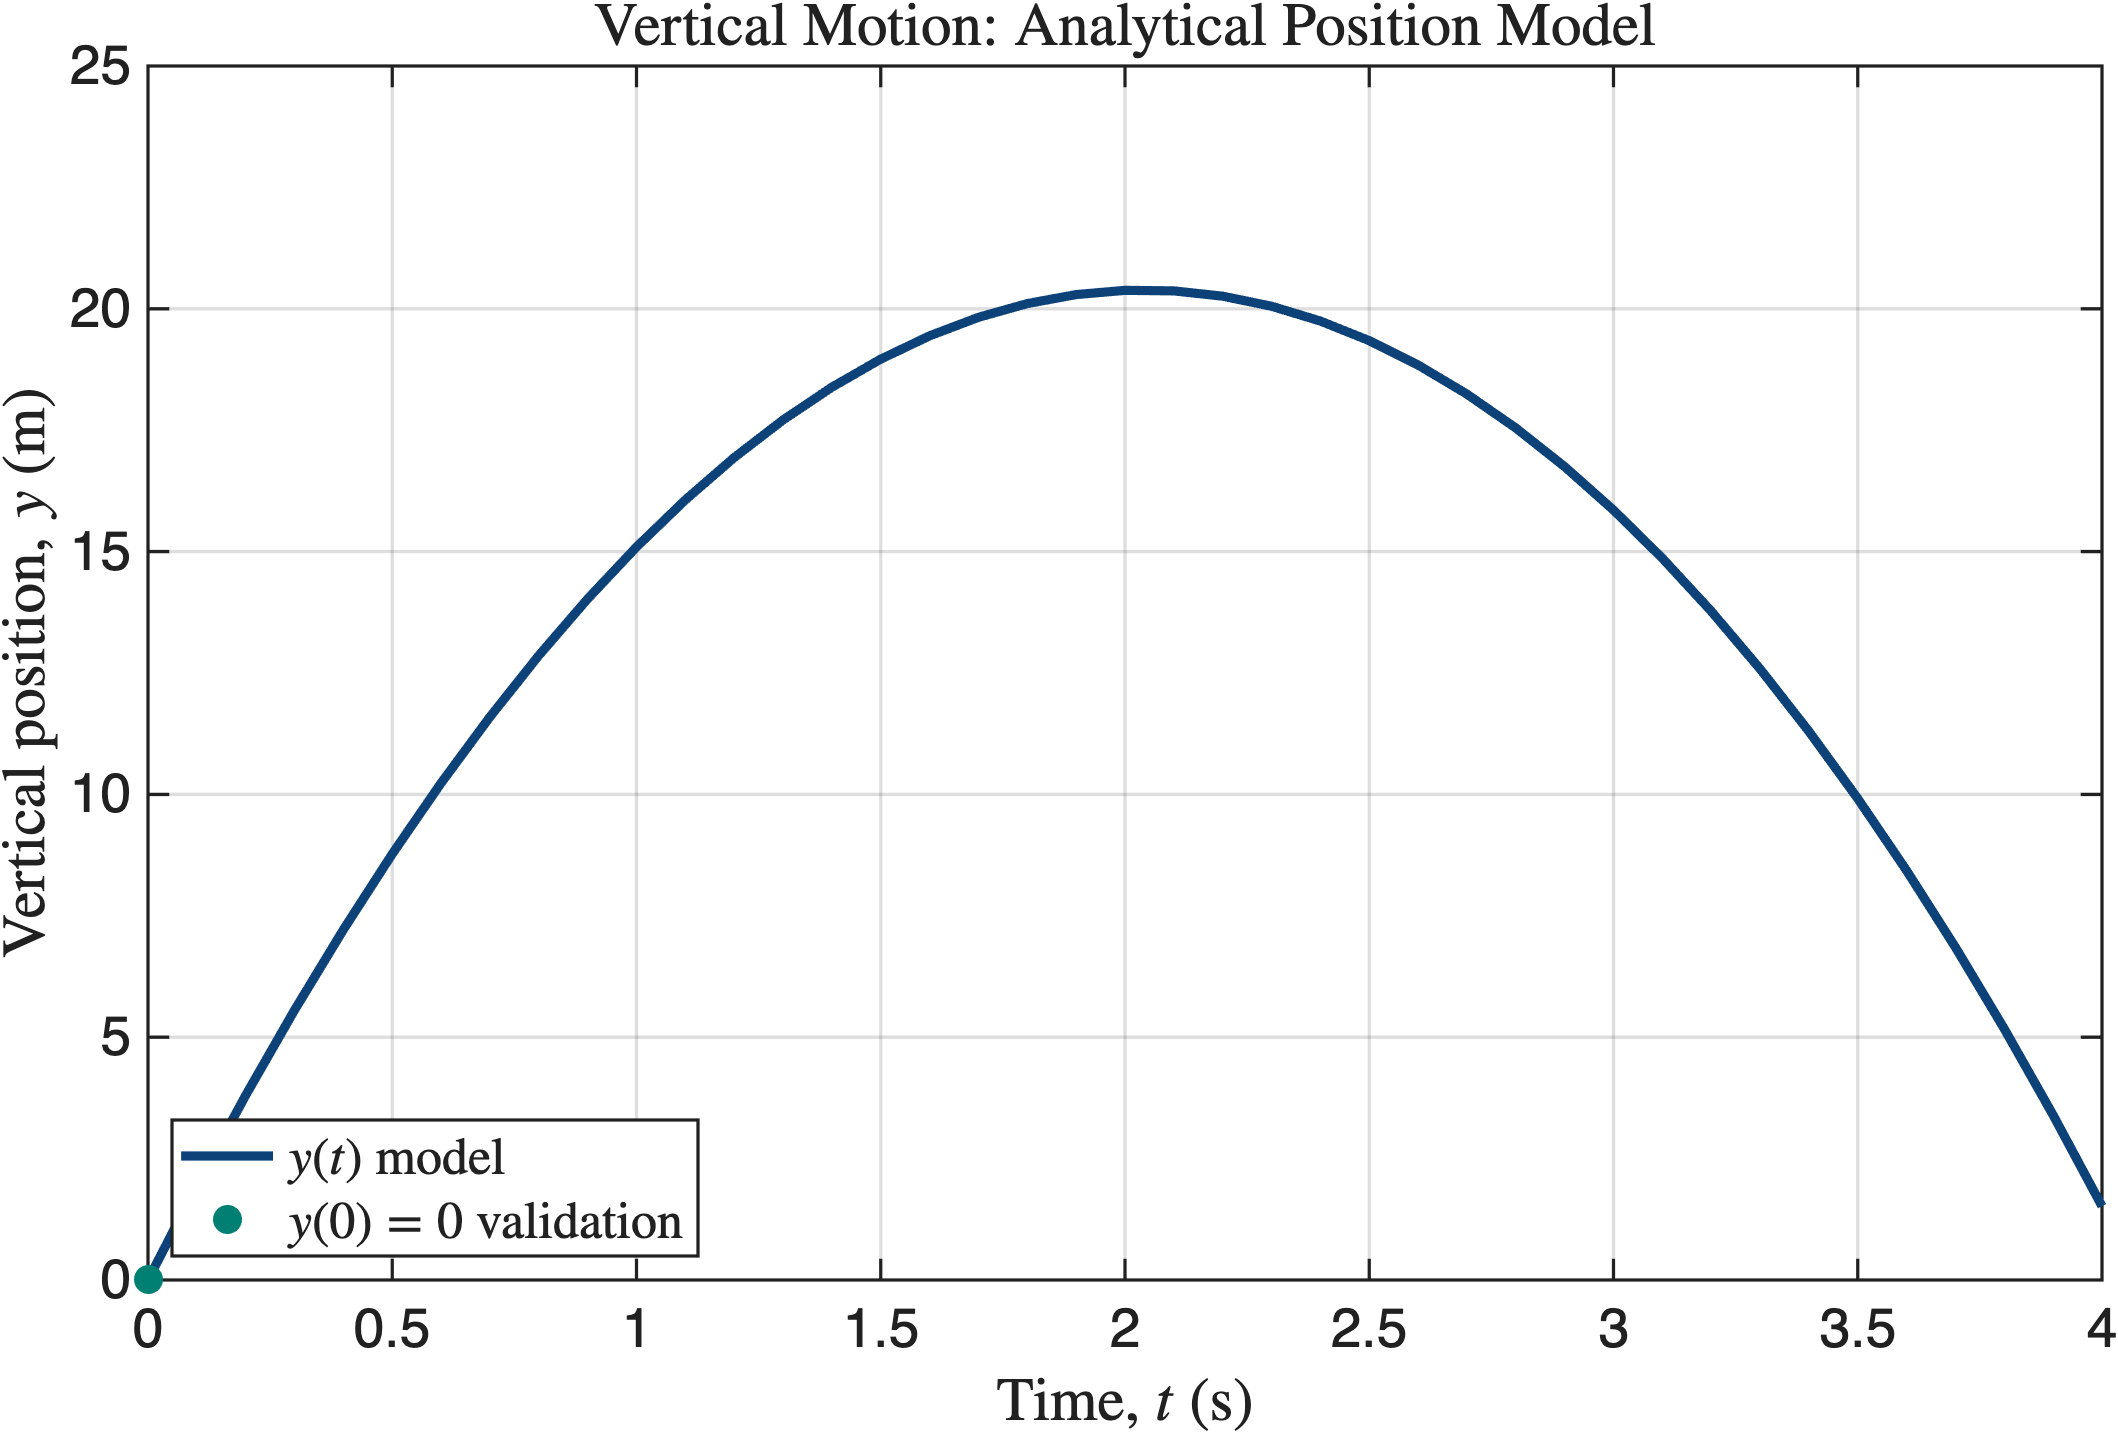
\includegraphics[width=.92\linewidth]{../matlab/assets/week01_height_time.png}\caption{MATLAB-generated numerical evidence for the locked vertical-motion model. The teal marker identifies the known initial value.}\end{figure}
\section*{8. One Core validation check}
At $t=0$, the equation must reproduce the initial condition. This value is known before code is run.
\begin{lstlisting}[style=matlabstyle,caption={Executable initial-value validation}]
assert(abs(y_m(1)-y0_m) < 1e-12,...
    'Initial-position validation failed.')
\end{lstlisting}
\begin{checkbox}\textbf{Validation result.} The first array entry is $y(0)=0\units{m}$, matching $y_0=0\units{m}$. The executable assertion passes from a fresh MATLAB session.\end{checkbox}
\section*{9. Interpret, troubleshoot, and communicate}
\begin{center}\small\begin{tabular}{>{\raggedright\arraybackslash}p{.35\linewidth}>{\raggedright\arraybackslash}p{.53\linewidth}}\toprule \textbf{If you see this} & \textbf{First check}\\ \midrule
The curve does not start at 0 m & Is \texttt{y0\_m = 0}, and are you looking at \texttt{y\_m(1)}?\\
A matrix-power error & Did \texttt{t\_s\string^2} need to be \texttt{t\_s.\string^2}?\\
The graph cannot answer the question & Add a title, labelled axes, and SI units.\\
The curve rises forever & Check the minus sign and the upward-positive convention.\\
The script changes between runs & Restart MATLAB and run all sections from the top.\\ \bottomrule\end{tabular}\end{center}
\section*{Working exposure: selected values and animation}
The lecture demonstration includes a lecturer-controlled animation of the same vertical launch. Its supplied loop only reveals the already-computed arrays in time order; writing loops is introduced as Core work in Week 2. The animation changes neither the equation, parameters, validation, nor physical conclusion.
\section*{Three takeaways}
\begin{enumerate}[nosep,leftmargin=6mm]\item A meaningful MATLAB name preserves a physical quantity and its unit. \item An array lets one familiar equation answer the same question at many times. \item A labelled graph becomes credible evidence when it agrees with a prediction and a known-value check.\end{enumerate}
\begin{keybox}\textbf{Preparation for the practical.} Open the lecture demonstration in MATLAB R2025a or later. Be ready to identify \texttt{t\_s(1)}, explain \texttt{t\_s.\string^2}, and state why $y(0)=0\units{m}$ is a valid check.\end{keybox}
\end{document}
